\documentclass[aspectratio=169,10pt
%	,handout
]{beamer}
%UnlimitedFonts
	\def\hmmax{0}
	\def\bmmax{0}
%SVG
	\usepackage{svg}
%Tables
	\usepackage{array,booktabs,tabularx,multirow}
	\newcolumntype{C}[1]{>{\hsize=#1\hsize%
		\centering\arraybackslash}X}
%Math&Fonts
	\let\latexointop\ointop
	\usepackage{mathtools,amssymb,bm % basics
		,physics,siunitx,slashed % physics
		,esint,nicefrac,extarrows,mathrsfs % more symbols
		,calligra,romannum,dsfont,fourier-orns % nice fonts
		,eqnarray,resizegather,empheq % more envs
		,relsize,stackengine % utils
	}
%	\usepackage{amsthm}
	\usepackage[scr=esstix]{mathalfa}
	\usepackage[only,sslash]{stmaryrd}
	%DisplaySetup
	\newcommand*\bbox[1]{\fbox{\hspace{1em}\addstackgap[5pt]{#1}\hspace{1em}}}
	\empheqset{box=\bbox}
	\mathtoolsset{showonlyrefs}
%Utils
	%Legacy \oint
	\let\ointop\undefined
	\let\ointop\latexointop
	%Calligra
	\DeclareMathAlphabet{\mathcalligra}{T1}{calligra}{m}{n}
	\DeclareFontShape{T1}{calligra}{m}{n}{<->s*[2.2]callig15}{}
	%CosmeticTweaks
	\newcommand\inlineeqno{\stepcounter{equation}\ (\theequation)}
	\newcommand\scalemath[2]{\scalebox{#1}{\mbox{\ensuremath{\displaystyle #2}}}}
	\newcommand\raisemath[2]{\raisebox{#1\depth}{${#2}$}}
	\newfontfamily\signature{Vladimir Script}
	\newcommand{\newparagraph}{\pagebreak[3]
		\noindent\hfil%
		\raisebox{-4pt}[10pt][10pt]{\leafright~\qquad~\leafleft}%
		\par\nopagebreak%
	}
%CustomCmds
	%Brackets
	\DeclarePairedDelimiter\ave{\langle}{\rangle}
	\DeclarePairedDelimiterX\inprod[2]{\langle}{\rangle}{#1,#2}
	%Basics
	\newcommand{\mbb}[1]{\mathbb{#1}}
	\newcommand{\mrm}[1]{\mathrm{#1}}
	\newcommand{\mcal}[1]{\mathcal{#1}}
	\newcommand{\mscr}[1]{\mathscr{#1}}
	\newcommand{\tup}[1]{\textup{#1}}
	\newcommand{\mop}[1]{\operatorname{#1}}
	%Extras
	\newcommand{\scriptr}{\mathcalligra{r}\,}
	\newcommand{\rvector}{\pmb{\mathcalligra{r}}\,}
	\newcommand{\hodgedual}{\operatorname{\star}}
	\newcommand{\dual}{\ \xlongleftrightarrow{\ \textrm{dual}\ }\ }
	\newcommand{\idty}{\mathds{1}}
	\newcommand{\proj}[1]{\operatorname{%
		proj_{\mathit{#1}}}}
	\newcommand{\propsim}{\mathbin{\ensurestackMath{
		\stackunder[2pt]{\propto}{\sim}
	}}}
	\newcommand{\textbox}[1]{\fbox{#1}}
	\newcommand{\pdd}[1]{\operatorname{\partial_{\mathnormal{#1}}}}
	\newcommand{\cdd}{\operatorname{D}\!}
	\newcommand{\cdv}[1]{\operatorname{%
		\nabla_{\!\mathit{#1}\!}}}
	\newcommand{\ldv}[1]{\operatorname{%
		\mcal{L}_{\!\mathit{#1}\!}}}
	\newcommand{\ric}[1]{\operatorname{%
		Ric}\!\pqty{#1}}
%Hacks
	% physics.sty <texmf-dist/tex/latex/physics/>
	% USER: more spacing around Dirac's middle vert
	\newcommand{\xmiddle}[1]{\mspace{1mu}\middle#1\mspace{1mu}}
	\DeclareDocumentCommand\innerproduct{ s m g }
	{ % Inner product
		\IfBooleanTF{#1}
		{ % No resize
			\IfNoValueTF{#3}
			{\vphantom{#2}\left\langle\smash{#2}\xmiddle\vert\smash{#2}\right\rangle}
			{\vphantom{#2#3}\left\langle\smash{#2}\xmiddle\vert\smash{#3}\right\rangle}
		}
		{ % Auto resize
			\IfNoValueTF{#3}
			{\left\langle{#2}\xmiddle\vert{#2}\right\rangle}
			{\left\langle{#2}\xmiddle\vert{#3}\right\rangle}
		}
	}


%Miscellaneous
	\newcommand{\naItl}{\tup{NaI\,(Tl)}}
	\newcommand{\csAtom}{${}^{137}\mrm{Cs}$}
	\newcommand{\coAtom}{${}^{60}\mrm{Co}$}
%Title
	\title{利用Notebook计算研究光电相互作用}
	\subtitle{基于实验:\naItl 闪烁谱仪测定$\gamma$射线的能谱}
	\author{\sffamily
		北京大学物理学院\ \textkai{Bryan}\\[.6ex]
		\ttfamily
		No.\,1500066666 | \scriptsize \url{masked_email_please_contact@github.com}
		\vspace{-1ex}
	}
	\institute{\large\ccbyncsajp}
	\date{}

\begin{document}
{%%% TITLEPAGE
\setbeamercolor{title in head/foot}{
		use=palette quaternary
		,fg=palette quaternary.bg
	}
\logo{}
\begin{frame}
	\titlegraphic{%
		\vspace{.05\textheight}
		\hspace{-.3\textwidth}
		\justify
		\noindent\scriptsize * Image courtesy: \\[.5ex]
		\noindent\url{https://www.sciencedirect.com/topics/medicine-and-dentistry/compton-scattering}
		\vspace{1\textheight}
	}
	\tikz [remember picture,overlay]
	\node at ([
		yshift=-3.2\baselineskip,xshift=-.25\linewidth
	] current page.east) {
		\begin{minipage}{.35\textwidth}
			\raggedright
			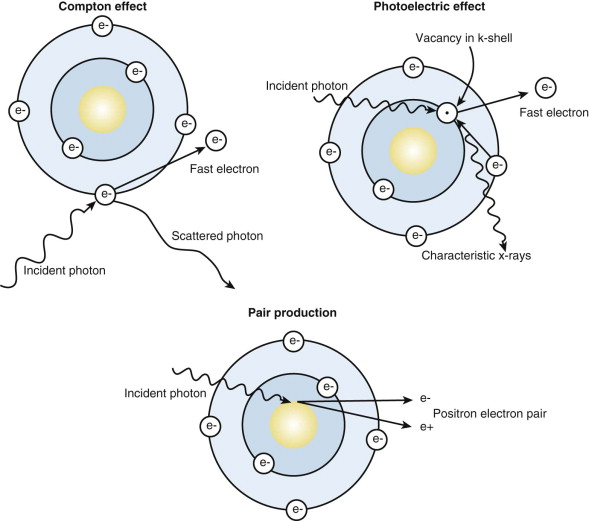
\includegraphics[
				width=\textwidth
			]{figs/photon_electron.jpg}
		\end{minipage}
	};
	\titlepage
\end{frame}
}%%% TITLEPAGE


\section*{引言}
\subsection{工具}
% beamer frame cannot handle \newcommand
% ... unless using ####1
\newcommand{\includeicon}[1]{
	\begin{minipage}[c][3em][c]{2em}
		\includegraphics[width=\linewidth]{figs/#1_logo.pdf}
	\end{minipage}
}
\begin{frame}{Notebook计算简介}{代码 + 图像 + 文档的数据处理环境}
	\vspace{-.35\baselineskip}
	\linespread{1.1}\selectfont%
%	\hspace{1em}~
	\begin{tabularx}{.65\linewidth}{C{1} C{1}}
	\toprule
%	\midrule
		\textbf{界面} / Front End & \textbf{后端} / Kernel \\
	\toprule%\midrule
		\includeicon{mathematica}
		Mathematica\texttrademark & Wolfram\texttrademark \\
	\midrule
		\multirow{5}{*}{%
			\includeicon{jupyter}
			Jupyter
		} & R \\
			& Python (NumPy, SciPy, ...) \\
			& Julia \\
			& CERN ROOT (C++) \\
			& $\cdots$ \\
	\midrule
		\multicolumn{2}{c}{
			\begin{minipage}[c][3em][c]{.5\linewidth}
				\centering
				
\includegraphics[height=2em]{figs/sage_logo.png}
			\end{minipage}
		} \\
%	\midrule
	\bottomrule
	\end{tabularx}
\end{frame}


\section{理论}
\subsection{探测原理}
\nologo{
\begin{frame}{闪烁体探头}{%
	$\gamma$光子
	$\longrightarrow$激发电子
	$\xrightarrow{\tup{\ 退激\ }}$闪烁光子(\naItl: $\sim\SI{415}{\nm}$蓝光)
	$\longrightarrow$光电倍增
}
	\begin{figure}[!ht]
		\centering
		\includesvg[width=.9\linewidth]{../img/PhotoMultiplierTubeAndScintillator.svg}
%		\hfil\vspace{1.5ex}
		\label{fig:NaIdetector}
%		\vspace{-1\baselineskip}
	\end{figure}
\end{frame}
}


\subsection{相互作用}
\begin{frame}{$\gamma$射线$E_\gamma$与闪烁体的相互作用}{
	考虑 \csAtom 源:$E_\gamma = \SI{.662}{\MeV}$
}
	\begin{enumerate}
	\item \textbf{光电效应:}$
		E = E_\gamma - E_i \simeq E_\gamma
		\simeq \SI{.662}{\MeV},\ E_i\ll E_\gamma
	$. 
	\item \textbf{Compton散射:}
	\begin{equation}
		E_{\gamma'} = E_\gamma \bigg/ \pqty\Big{
			1 + \alpha\,(1 - \cos\theta)
		},\quad
		\alpha = \frac{E_\gamma}{m_e c^2}
	\end{equation}
	$E = E_\gamma - E_{\gamma'}$随散射角$\theta\in\bqty{0,\pi}$递增,
	\begin{equation}
		E_{\max} = E_\gamma\,\frac{2\alpha}{1 + 2\alpha}
		\simeq \SI{.478}{\MeV}
	\end{equation}
	{\smaller
	* 反散射 + 光电效应$\to$反散射峰$
		E_{\gamma'}
		= E_\gamma - E_{\max}
		\simeq \SI{.184}{\MeV}
	$. }
	\item \textbf{正负电子对产生(然后湮灭):}$m_e c^2 \simeq \SI{.511}{\MeV}$
	\\[1ex]
	\smaller
	* 对 \csAtom 源$E_\gamma < 2m_e c^2$不会产生
	\end{enumerate}
\end{frame}


\nologo{
\begin{frame}{Compton能谱}{
	如何定量地得到Compton能谱?
}
	\vspace*{-.5\baselineskip}
	\begin{center}
		\raisebox{-.5\height}{
			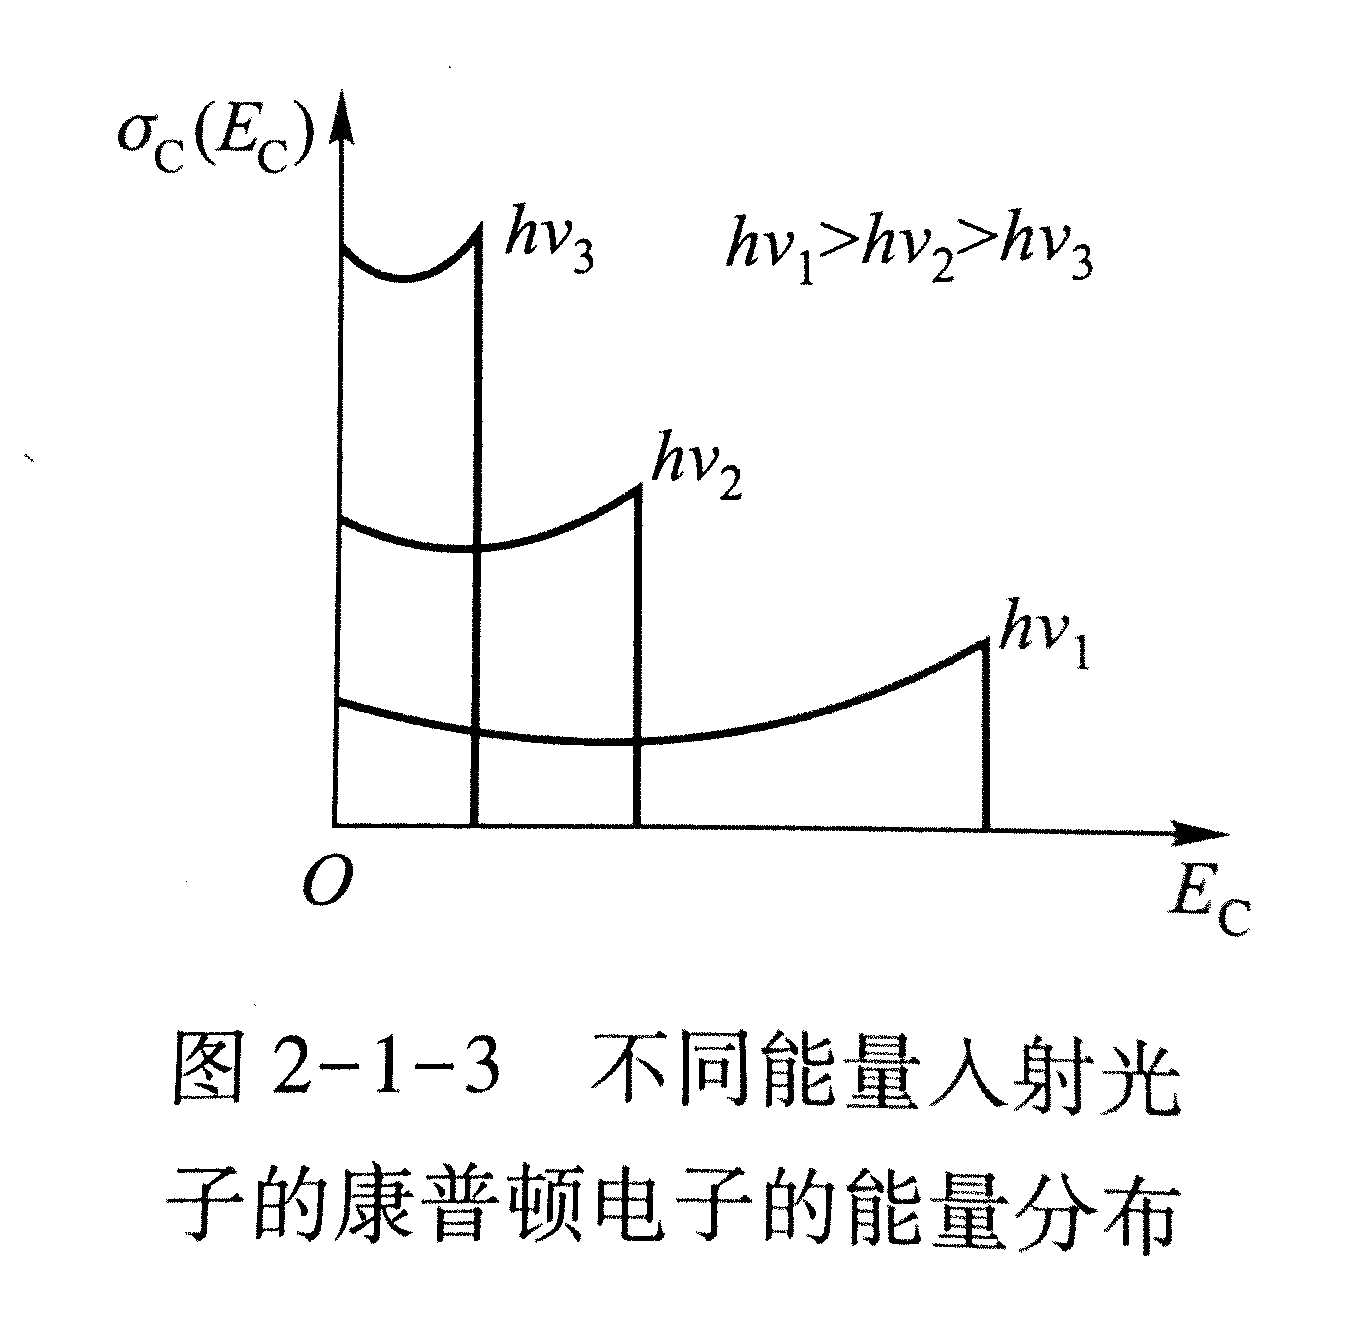
\includegraphics[width=.435\linewidth]{figs/spectrum_compton.png}
		}
		\raisebox{-.5\height}{
			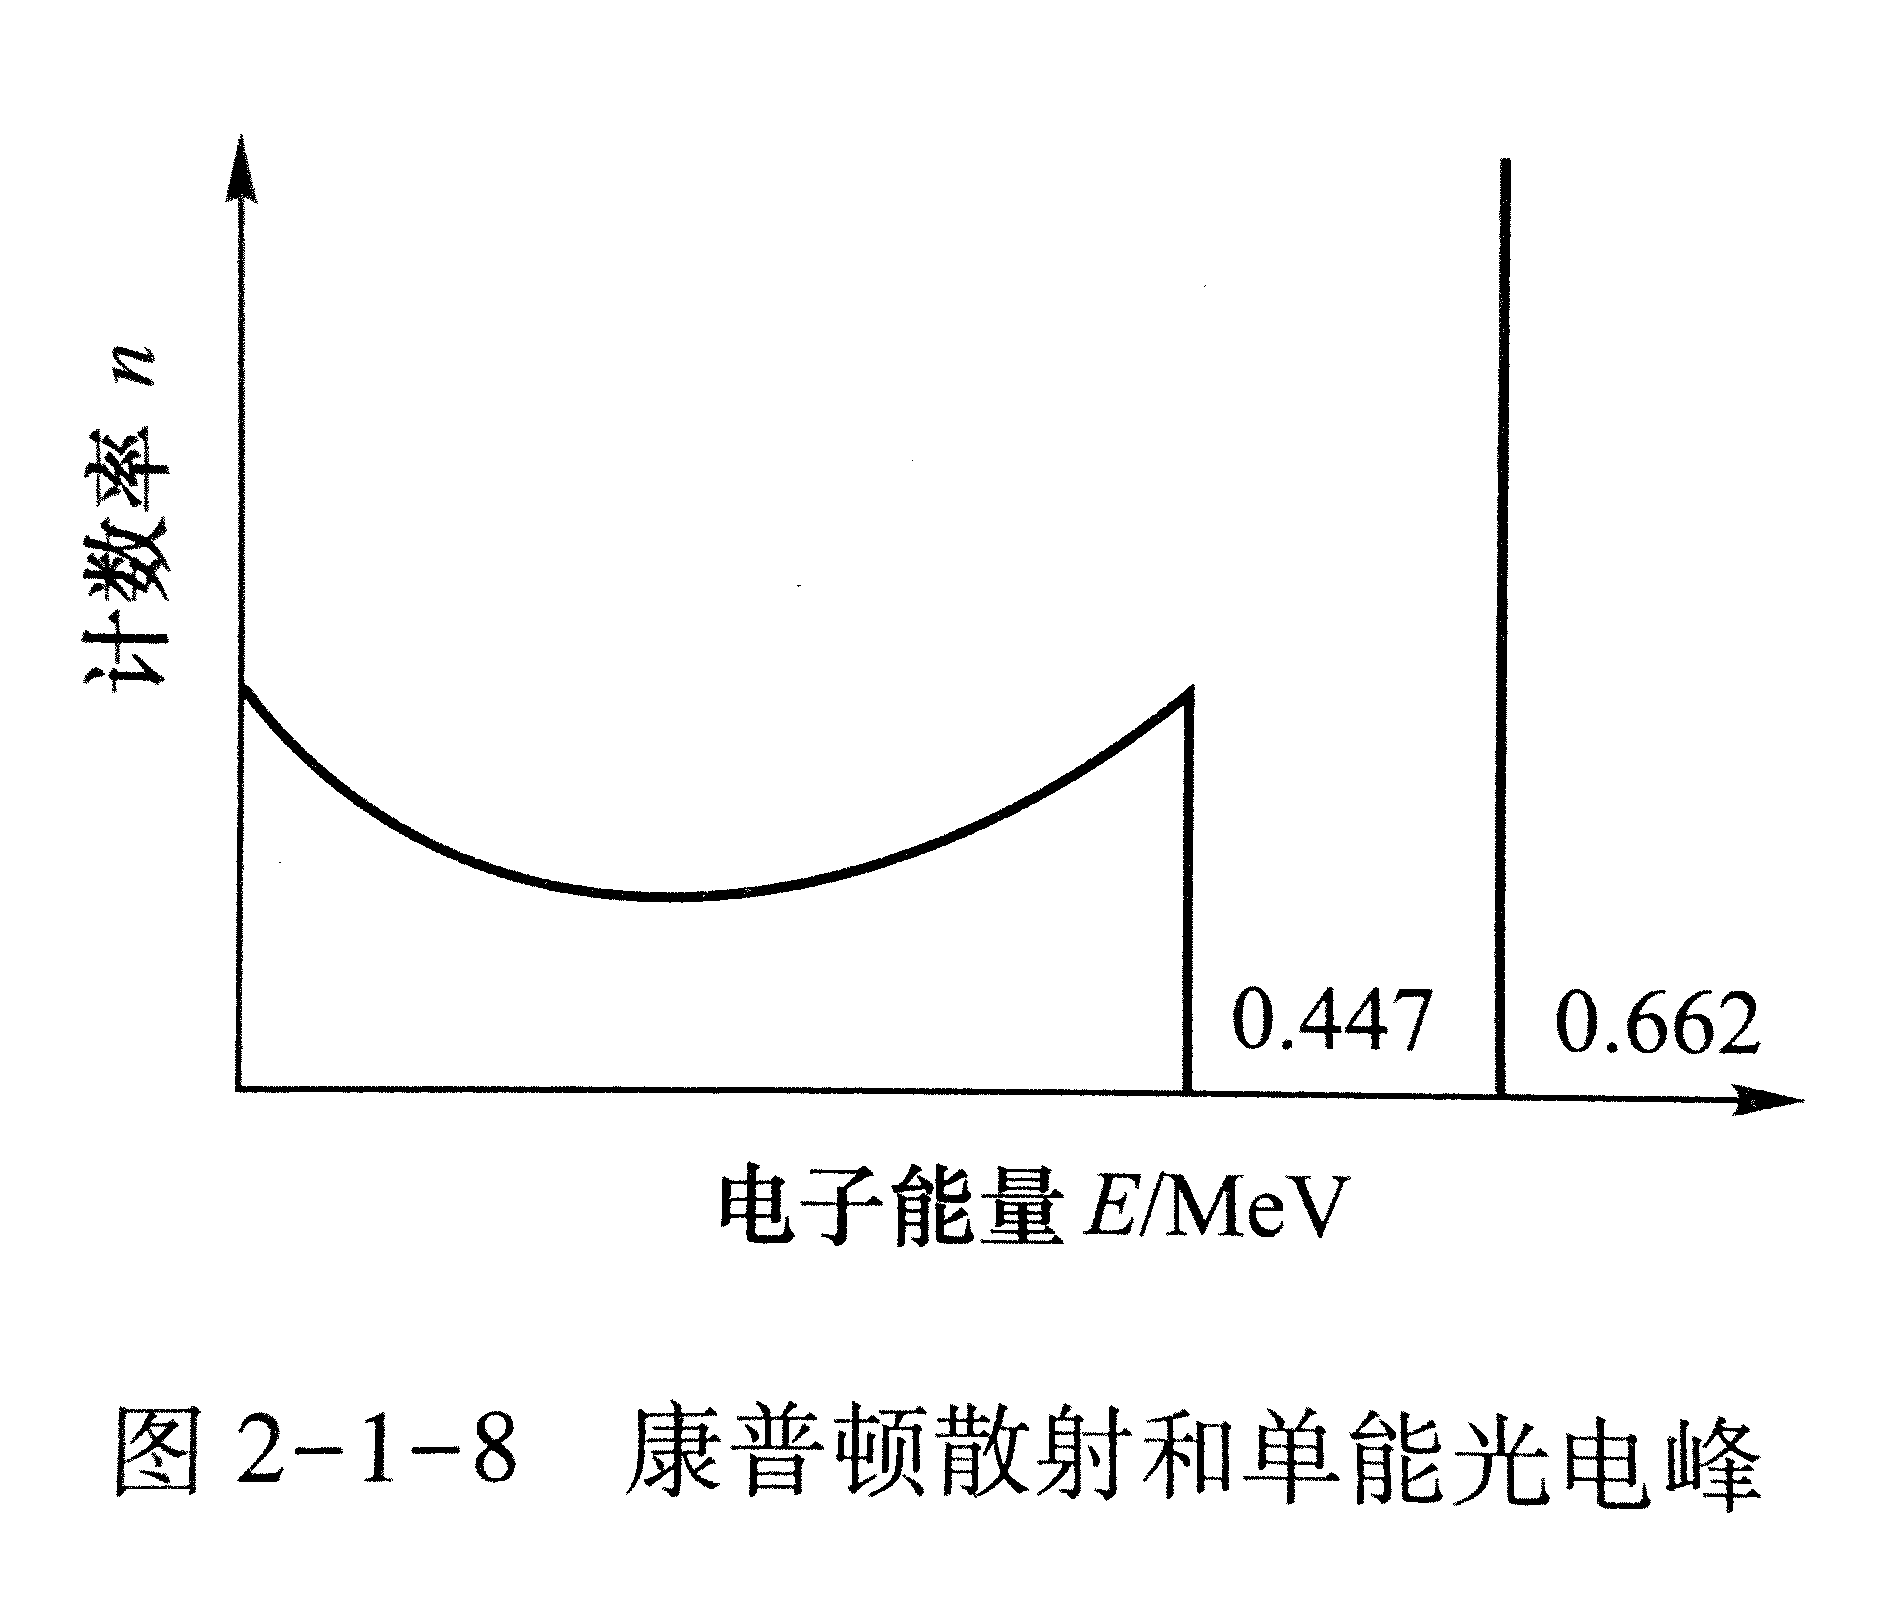
\includegraphics[width=.435\linewidth]{figs/spectrum_full.png}
		}
%		\hfil\vspace{1.5ex}
%		\label{fig:NaIdetector}
%		\vspace{-1\baselineskip}
	\end{center}
	\tikz [remember picture,overlay]
	\node at ([
		yshift=-.035\textheight,xshift=-.395\linewidth
	] current page.east) {
		
\includegraphics[width=3.5em]{figs/confused.png}
	};
\end{frame}
}


\nologo{
\begin{frame}{Klein–Nishina公式}{
	QED的最早结果之一(由半经典方法得到);
	时间点:Schrödinger 1926, Dirac 1928
}
%	\vspace*{-.5\baselineskip}
	\begin{minipage}{.5\linewidth}
		\begin{itemize}
		\item $p = \frac{E_{\gamma'}}{E_\gamma} = \frac{1}{1 + \alpha\,(1 - \cos\theta)}$, 
			\begin{equation}
				\dv{\sigma}{\Omega}
				\propto p^2 \pqty\big{p + p^{-1} - \sin^2\theta} \Big/ 2
			\end{equation}
		\item $\alpha = \frac{E_\gamma}{m_e c^2}\to 0$时,$p\to 1$, \\[.5ex]
			回归经典Thomson散射$
				\dv{\sigma}{\Omega}
				\propto\frac{1 + \cos^2\theta}{2}
			$. 
		\item 图片源自Wikipedia.
		\end{itemize}
	\end{minipage}
	\quad
	\begin{minipage}{.4\linewidth}
		\includegraphics[width=\linewidth]{../img/Klein-Nishina_distribution.png}
	\end{minipage}
\end{frame}
}


\begin{frame}{Compton谱线理论计算}{}
	\vspace*{-.5\baselineskip}
	\begin{itemize}
	\item 截面关于$E$的分布:
	\begin{equation}
		\dv{\sigma}{E}
		= \dv{\sigma}{\theta} \bigg/ \dv{E}{\theta}
		= 2\pi\sin\theta\,\dv{\sigma}{\Omega} \bigg/ \dv{E}{\theta}
		\label{eq:comptonSectionByEnergy}
	\end{equation}
	$E = E_\gamma\pqty\big{
		1 - \frac{1}{1 + \alpha\,(1 - \cos\theta)}
	}$,
	\item 定性分析:
	\begin{itemize}
	\item $E = 0, E_{\max}$处$\dv{E}{\theta} = 0$, 据 \eqref{eq:comptonSectionByEnergy} 可见,对应能谱上的峰值
	\item $0 < E < E_{\max}$大致为低于左右峰值的平台
	\end{itemize}
	\end{itemize}
\end{frame}


\nologo{
\begin{frame}{数值计算Compton能谱}{
	\href{run:../data/theory.nb}{[Mathematica计算]},
	有限能量分辨带来的展宽:与$\sigma = \num{.01}$正态分布卷积
}
%	\vspace*{-.5\baselineskip}
	\begin{itemize}
	\item Mathematica的独特优势:代数计算
	\end{itemize}
	\newcommand{\figwidth}{.485\linewidth}
	\noindent%
	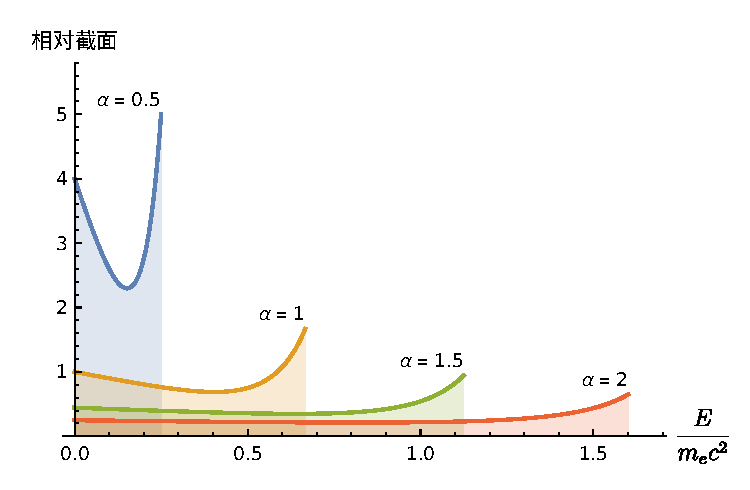
\includegraphics[width=\figwidth]{../img/plots/comptonSpectrum.pdf}
	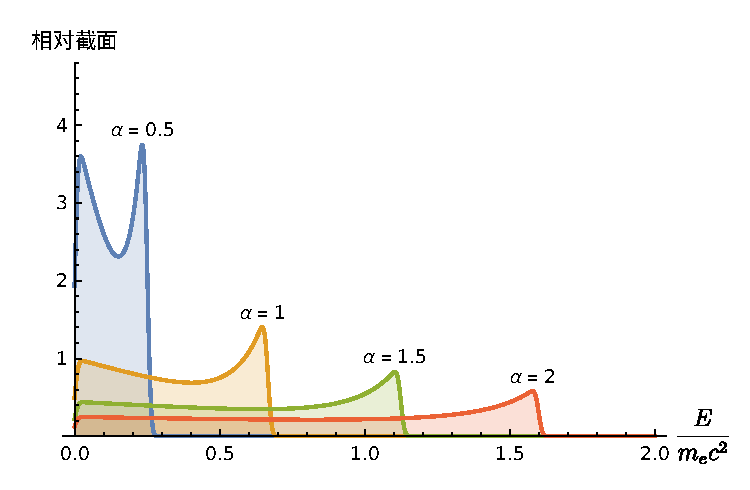
\includegraphics[width=\figwidth]{../img/plots/comptonSpectrumObs.pdf}
\end{frame}
}


\section{实验}
\subsection{测定能谱}
\begin{frame}{单道:逐点测定全谱}{
	有多道了,为何还要用单道?付老师答曰:体验一下...
}
%	\vspace*{-.5\baselineskip}
	\begin{itemize}
	\item 阈值$V$, 道宽$\Delta V$, 计数$V\sim V + \Delta V$, \\[.2ex]
		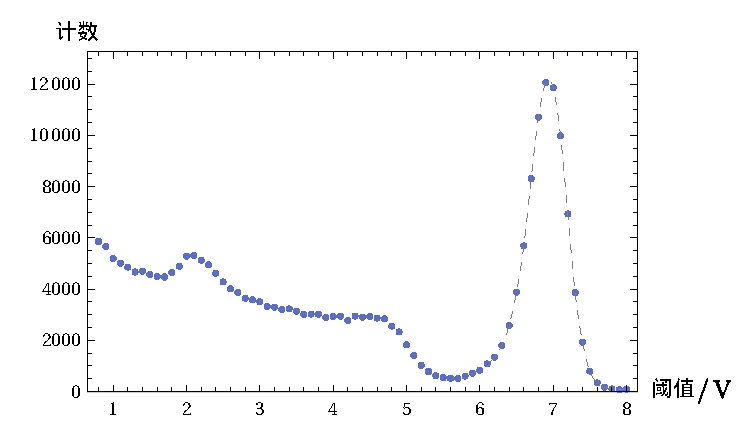
\includegraphics[height=.65\textheight]{../img/plots/spectrumPlot.pdf}
	\end{itemize}
\end{frame}


\begin{frame}[fragile]{Notebook可视化流程(\textit{Workflow})}{
%	有多道了,为何还要用单道?付老师答曰:体验一下...
}
%	\vspace*{-.5\baselineskip}
	\begin{itemize}
	\item 在数据表(如 \tup{Excel})中记录数据,文件名 \texttt{data.ods}
	\item Mathematica可视化追踪:
%
\begin{minted}{mathematica}
Import["data.ods"][[1]] // ListPlot
\end{minted}
%
	\item 分析:
		\begin{itemize}
		\item 能量刻度:寻峰 \verb|FindPeaks|, 线性回归 \verb|LinearModelFit|
		\item 能量分辨:插值 \verb|Interpolation|, 求根 \verb|FindRoot| 得半宽
		\end{itemize}
	\end{itemize}
\end{frame}


\begin{frame}{多道:一步到位}{
	多道与单道的结果在低能端不甚一致,原因未知
}
%	\vspace*{-.5\baselineskip}
	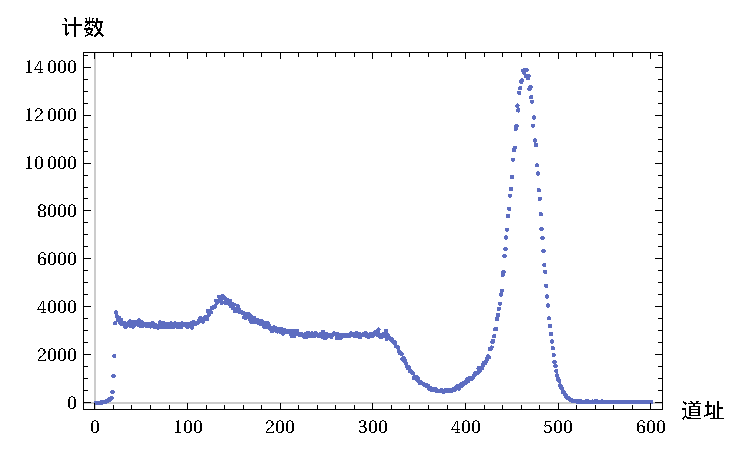
\includegraphics[height=.75\textheight]{../data/plots/csSpectrumTruncated.pdf}
\end{frame}


\section{结语}
\subsection{核心观点}
\begin{frame}{总结}
%	\vspace*{-.5\baselineskip}
	\begin{itemize}
	\item Compton能谱的形态:微分散射截面
	\item Notebook计算在实验中的应用:
		\begin{itemize}
		\item Mathematica的独特优势:符号计算\\[.5ex]
			\quad Compton能谱的具体形式:\\[1.ex]
			\qquad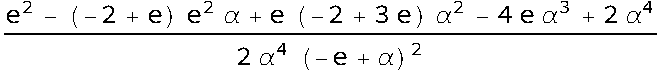
\includegraphics[width=.5\linewidth]{../data/comptonSectionByEnergyOut.pdf}
		\item Notebook界面的共同特点:快速可视化 + 代码可重复
		\end{itemize}
	\end{itemize}
\end{frame}


\begin{frame}{致谢}
	\Huge
	\noindent
	\raisebox{-.5\height}{
		
\includegraphics[width=.4\linewidth]{figs/hilarious.jpg}
	}
	\quad 谢谢大家!
\end{frame}

%	\animategraphics[loop,width=.235\linewidth]{7}{figs/2hamiltonianFlow/2hamiltonianFlow-}{1}{85}
\end{document}